\documentclass[unicode,11pt,a4paper,oneside,numbers=endperiod,openany]{scrartcl}

\usepackage{ifthen}
\usepackage[utf8]{inputenc}
\usepackage{graphics}
\usepackage{graphicx}
\usepackage{hyperref}

\pagestyle{plain}
\voffset -5mm
\oddsidemargin  0mm
\evensidemargin -11mm
\marginparwidth 2cm
\marginparsep 0pt
\topmargin 0mm
\headheight 0pt
\headsep 0pt
\topskip 0pt        
\textheight 255mm
\textwidth 165mm

\newcommand{\duedate} {}
\newcommand{\setduedate}[1]{%
\renewcommand\duedate {Due date:~ #1}}
\newcommand\isassignment {false}
\newcommand{\setassignment}{\renewcommand\isassignment {true}}
\newcommand{\ifassignment}[1]{\ifthenelse{\boolean{\isassignment}}{#1}{}}
\newcommand{\ifnotassignment}[1]{\ifthenelse{\boolean{\isassignment}}{}{#1}}

\newcommand{\assignmentpolicy}{
\begin{table}[h]
\begin{center}
\scalebox{0.8} {%
\begin{tabular}{|p{0.02cm}p{16cm}|}
\hline
&\\
\multicolumn{2}{|c|}{\Large\textbf{HPC Lab for CSE 2024 ---  Submission Instructions}}\\
\multicolumn{2}{|c|}{\large\textbf{(Please, notice that following instructions are mandatory: }}\\
\multicolumn{2}{|c|}{\large\textbf{submissions that don't comply with, won't be considered)}}\\
&\\
\textbullet & Assignments must be submitted to \href{https://moodle-app2.let.ethz.ch/course/view.php?id=22516}{Moodle} (i.e. in electronic format).\\
\textbullet & Provide both executable package and sources (e.g. C/C++ files, Matlab). 
If you are using libraries, please add them in the file. Sources must be organized in directories called:\\
\multicolumn{2}{|c|}{\textit{Project\_number\_lastname\_firstname}}\\
& and  the  file must be called:\\
\multicolumn{2}{|c|}{\textit{project\_number\_lastname\_firstname.zip}}\\
\multicolumn{2}{|c|}{\textit{project\_number\_lastname\_firstname.pdf}}\\
\textbullet &  The TAs will grade your project by reviewing your project write-up, and looking at the implementation 
                 you attempted, and benchmarking your code's performance.\\

\textbullet & You are allowed to discuss all questions with anyone you like; however: (i) your submission must list anyone you discussed problems with and (ii) you must write up your submission independently.\\
\hline
\end{tabular}
}
\end{center}
\end{table}
}
\newcommand{\punkte}[1]{\hspace{1ex}\emph{\mdseries\hfill(#1~\ifcase#1{Points}\or{Points}\else{Points}\fi)}}


\newcommand\serieheader[6]{
\thispagestyle{empty}%
\begin{flushleft}

\includegraphics[width=0.4\textwidth]{ETHlogo_13}
\end{flushleft}
  \noindent%
  {\large\ignorespaces{\textbf{#1}}\hspace{\fill}\ignorespaces{ \textbf{#2}}}\\ \\%
  {\large\ignorespaces #3 \hspace{\fill}\ignorespaces #4}\\
  \noindent%
  \bigskip
  \hrule\par\bigskip\noindent%
  \bigskip {\ignorespaces {\Large{\textbf{#5}}}
  \hspace{\fill}\ignorespaces \large \ifthenelse{\boolean{\isassignment}}{\duedate}{#6}}
  \hrule\par\bigskip\noindent%  \linebreak
 }

\makeatletter
\def\enumerateMod{\ifnum \@enumdepth >3 \@toodeep\else
      \advance\@enumdepth \@ne
      \edef\@enumctr{enum\romannumeral\the\@enumdepth}\list
      {\csname label\@enumctr\endcsname}{\usecounter
        {\@enumctr}%%%? the following differs from "enumerate"
	\topsep0pt%
	\partopsep0pt%
	\itemsep0pt%
	\def\makelabel##1{\hss\llap{##1}}}\fi}
\let\endenumerateMod =\endlist
\makeatother




\usepackage{textcomp}






\usepackage{minted}
\usepackage{amsmath}
\usepackage{listings}
\usepackage{subcaption}

\begin{document}


\setassignment
\setduedate{Monday 29 April 2024, 23:59 (midnight).}

\serieheader{High-Performance Computing Lab for CSE}{2024}
{Student: Benedict Armstrong}
{Discussed with: Tristan Gabl}{Solution for Project 4}{}
\newline

% \assignmentpolicy

\section{Ring sum using MPI [10 Points]}
For this task we are asked to implement a ring sum using MPI. We calculate the sum of all MPI ranks in a communicator. To do this each process starts by sending its rank to the next process in the ring adds it to an internal sum and then sends the message on to the next process. This is done until each message has made a full loop of the ring. We notice that by the end the sum should be equal to the sum of all ranks in the communicator.

$$
      \sum_{i=0}^{n-1} i = \frac{n(n-1)}{2}
$$


To avoid avoid deadlocks we can make every process send before they receive.


\section{Cartesian domain decomposition and ghost cells exchange [20 Points]}

The implementation of this task was relatively straightforward after doing the MPI tutorial. The main difficulty was not making any errors with the indexing into the data array. The convenient \texttt{MPI\_Cart\_shift} function makes it easy to get the rank of the cartesian up/down/left/right neighbors. To avoid deadlocks I used the asynchronous \texttt{MPI\_Isend} and \texttt{MPI\_Irecv} functions and then waited for all the communication to finish using \texttt{MPI\_Waitall} at the end.
For the diagonal neighbors I used the \texttt{MPI\_Cart\_coords} function to get the coordinates of the current rank and then added/subtracted 1 from each coordinate to get the coordinates of the diagonal neighbors. This was then converted back into a rank using \texttt{MPI\_Cart\_rank}. Running the program using \ref{lst:ghost_run} produces the output in \ref{lst:ghost_output}. For debugging purposes I also printed the neighbors of each rank. Below that we can see that the output data from rank 9 indeed matches the expected result outlined in the assignment.

\begin{listing}[h!t]
      \begin{minted}{bash}
      mpirun -np 16 ./build/ghost
      \end{minted}
      \caption{Running the ghost cell exchange program}
      \label{lst:ghost_run}
\end{listing}

\begin{listing}[h!t]
      \begin{minted}{bash}
      Neighbors of rank 9
      +-----------+
      |  4|  5|  6|
      |-----------|
      |  8|  9| 10|
      |-----------|
      | 12| 13| 14|
      +-----------+
      data of rank 9 after communication
      4  5  5  5  5  5  5  6 
      8  9  9  9  9  9  9 10 
      8  9  9  9  9  9  9 10 
      8  9  9  9  9  9  9 10 
      8  9  9  9  9  9  9 10 
      8  9  9  9  9  9  9 10 
      8  9  9  9  9  9  9 10 
      12 13 13 13 13 13 13 14 
      \end{minted}
      \caption{Output of the ghost cell exchange program}
      \label{lst:ghost_output}
\end{listing}


\section{Parallelizing the Mandelbrot set using MPI [30 Points]}

To start I implemented the partitioning as outlined in the assignment handout. The MPI documentation at \href{https://rookiehpc.org/mpi/docs/} was very helpful for this. After each process has calculated its part of the Mandelbrot set we need to gather the data back to the root process. This is implemented by simply receiving the data from each process in the root process (rank 0) and writing the data to a png file. There is no danger of a deadlock here as there are no dependencies between the processes. Only the root process writes the data to a file. The output image is shown in figure \ref{fig:mandelbrot}.

To evaluate the performance I ran the program with $p = 1, 2, 4, 8, 16$ processes and an image size of $4096 \times 4096$. Figure \ref{fig:mandelbrot_perf} shows the time taken by each processes (rank) for different number of processes.

\begin{figure}
      \centering
      
\includegraphics[width=.5\linewidth]{plots/mandel.png}
      \caption{Mandelbrot set}
      \label{fig:mandelbrot}
\end{figure}

\begin{figure}
      \centering
      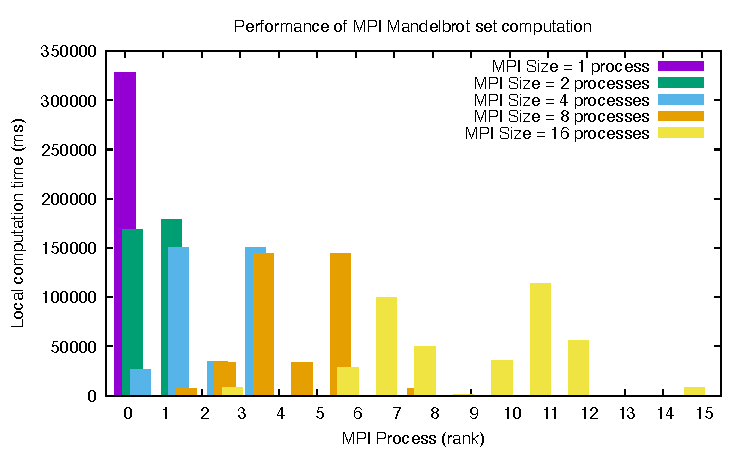
\includegraphics[width=.8\linewidth]{plots/mandel_perf.pdf}
      \caption{Performance of the Mandelbrot set program}
      \label{fig:mandelbrot_perf}
\end{figure}


\section{Parallel matrix-vector multiplication and the power method
        [40 Points]}


\end{document}
